\documentclass[12pt,a4paper]{book}
\usepackage[utf8]{inputenc}
\usepackage{amsmath}
\usepackage{amsfonts}
\usepackage{amssymb}
\usepackage{graphicx}
\usepackage[a4paper,margin=1in]{geometry}
\usepackage[frenchb]{babel}
\usepackage[autolanguage]{numprint}
\usepackage{xspace}
\usepackage{ragged2e}
\sloppy

\begin{document}
	\section*{Introduction}
	La spectroscopie vibrationnelle fournit de nombreuses informations sur la structure des matériaux. Dans le cas, des structures cristallines où l'interprétation des spectres expérimentaux est très difficile en raison de l'influence du champ cristallin sur les motifs, c'est possible éliminer ces difficultés par l'utilisation en parallèle de deux méthodes spectroscopiques: les spectroscopies Raman et Infrarouge. \\
	
	En effet, la spectroscopie Raman et la spectroscopie Infrarouge sont des techniques expérimentales complémentaires, flexibles et puissantes qui sont utilisées dans la caractérisation de matériaux. Elles donnent des informations directes sur la surface d'énergie potentielle au voisinage de la position d'équilibre et permet ainsi un examen des caractéristiques structurales des systèmes étudies. Cependant, dans le pratique, l'analyse et l'attribution des données du spectre sont difficiles, ce qui conduit souvent l'expérimentateur à se focaliser sur les caractéristiques de groupes fonctionnels et des familles de bandes associées. Une perte de certaines informations données par le spectre est donc inéluctable. \\
		
	Les méthodes ab initio apportent une solution à ce problème dans une certaine mesure, en déterminant précisément le spectre vibrationnelle d'un système. Il est alors possible d'attribuer sans équivoque les données issues du spectre aux modes normaux d'oscillation correspondant, rendant ainsi possible une meilleure compréhension du spectre vibrationnel, ainsi qu'une meilleure caractérisation des propriétés chimiques du système considéré. Des alors qu'il sera possible de réaliser de manière routinière des calculs de type ab initio de haute qualité sur des systèmes de plus en plus complexes, cela permettra potentiellement aux expérimentateurs de réaliser des analyses complémentaires de plus en plus fiables du spectre obtenu. 
	
		
\section{Dynamique du réseau cristallin: Hypothèses fondamentales}
	
	Comme point de départ, nous considérons une maille élémentaire d'un cristal parfait, n'étant soumis à aucune vibration. Le réseau de Bravais correspondant est constitué de tous les points décrits par les vecteurs $\overrightarrow{R}$ tel que:
	
	\begin{equation}
	\overrightarrow{R}= n_{1}\overrightarrow{a_{1}} + n_{2}\overrightarrow{a_{2}} + n_{3}\overrightarrow{a_{3}}
	\end{equation}
	
Où,$\overrightarrow{a_{1}}, \overrightarrow{a_{2}}, \overrightarrow{a_{3}}$ sont les vecteurs primitifs de la maille élémentaire et $n_{i}\in Z$. La position $\overrightarrow{r_{j}}$ d'un atome j à sa position d'équilibre dans la cellule primitive spécifiée par $\overrightarrow{R}$ est donnée par:	

\begin{equation}
\overrightarrow{r_{j}} (\overrightarrow{R}) = \overrightarrow{R} + \overrightarrow{d_{j}}
\end{equation}

La position de l'atome j soumis à des vibrations est donnée par:

\begin{equation}
\overrightarrow{r_{j}} (\overrightarrow{R}) = \overrightarrow{R} + \overrightarrow{d_{j}} + \overrightarrow{u_{j}}(\overrightarrow{R})
\end{equation}	

Où $\overrightarrow{u_{j}}(\overrightarrow{R})$ représente le déplacement de l'atome j par rapport à la position d'équilibre L'hypothèse de l'amplitude de déplacement $\overrightarrow{u}(\overrightarrow{R})$ faible sera admise dans tout ce qui va suivre, ceci permettant de considérer l'approximation harmonique. On précise cependant qu'une telle approche exclut l'étude de certaines propriétés comme par exemple, la diffusion d'un ion dans un cristal ou le comportement des solides à des températures proches de leur point de fusion. De la même façon, certaines propriétés, telles que la dilatation thermique et la conductibilité thermique, ne peuvent s'expliquer qu'en introduisant des termes anharmoniques.
\bigskip
Consideron, un cristal dans une base monoatomique, dans lequel on peut décrire l'énergie potentielle d'interaction entre les ions comme une somme d'interactions de paires. Soit $\phi(\overrightarrow{x})$ le potentiel d'interaction entre 2 ions sépares par le vecteur $\overrightarrow{x}$. Ce potentiel ne dépend que de la position relative des ions. En tenant compte des vibrations, on a: 
\begin{equation}
\overrightarrow{x}= \overrightarrow{R} - \overrightarrow{R'} + \overrightarrow{u}(\overrightarrow{R}) -\overrightarrow{u}(\overrightarrow{R'})
\end{equation}

\begin{figure}
	\centering
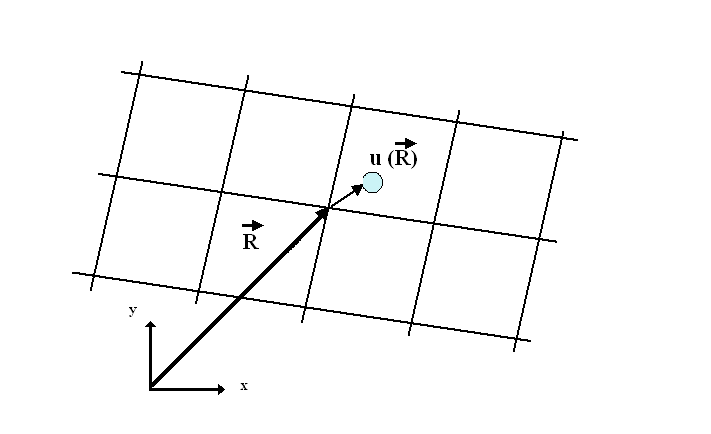
\includegraphics[scale=0.8]{reseauB}
\caption[Reseau de Bravais et veteur de déplacement pour une base monoatomique]{Réseau de Bravais et vecteur de déplacement u($\overrightarrow{R}$) pour une base monoatomique.}	
\end{figure}


L'énergie potentielle totale s'écrit donc:

\begin{equation}
U = \frac{1}{2} \sum_{\substack{\overrightarrow{R},\overrightarrow{R'}\\ \overrightarrow{R}\neq \overrightarrow{R'}}} \phi [\overrightarrow{R} - \overrightarrow{R'} + \overrightarrow{u}(\overrightarrow{R})- \overrightarrow{u}(\overrightarrow{R'})]
\end{equation}

Dans l'hypothèse où les déplacements $\overrightarrow{u}(\overrightarrow{R})$ sont faibles, on peut développer $\phi(\overrightarrow{x})$ autour de $(\overrightarrow{R}-\overrightarrow{R'})$, et on obtient (avec $\alpha$, $\beta$= x,y,z):

\begin{equation*}
U = \frac{1}{2}\sum_{\substack{\overrightarrow{R},\overrightarrow{R'}\\ \overrightarrow{R}\neq \overrightarrow{R'}}} \left\{\phi(\overrightarrow{R}-\overrightarrow{R'}) + \sum_{\alpha} [u_{\alpha}(\overrightarrow{R})- u_{\alpha}(\overrightarrow{R'})] \frac{\partial\phi}{\partial x_{\alpha}}\Big|_{\overrightarrow{R}-\overrightarrow{R'}}\right.
\end{equation*}
\begin{equation}
\left.+\frac{1}{2} \sum_{\alpha,\beta}[u_{\alpha}(\overrightarrow{R})-u_{\alpha}(\overrightarrow{R'})][u_{\beta}(\overrightarrow{R})-u_{\beta}(\overrightarrow{R'})] \frac{\partial^{2}\phi}{\partial x_{\alpha} \partial x_{\beta}}\Big|_{\overrightarrow{R}-\overrightarrow{R'}} + \ldots\right\} \label{equation1}
\end{equation}

Le premier terme de l'équation (\ref{equation1}) correspond au potentiel sans tenir compte des vibrations (réseau statique), il s'écrit:

\begin{equation}
U_{stat} = \frac{1}{2} \sum_{\substack{\overrightarrow{R},\overrightarrow{R'}\\ \overrightarrow{R}\neq \overrightarrow{R'}}} \phi(\overrightarrow{R}-\overrightarrow{R'}) = \frac{N}{2} \sum_{\overrightarrow{R}\neq0} \phi(\overrightarrow{R})
\end{equation}

Le terme linéaire de (\ref{equation1}) s'annule, le coefficient de $u_{\alpha}(\overrightarrow{R})$ correspondant à la somme des forces qui s'exercent sur l'ion R à l'équilibre

On a : 

\begin{equation}
\frac{1}{2} \sum_{\overrightarrow{R'}} \frac{\partial\phi}{\partial x_{\alpha}}\Big|_{\overrightarrow{R}-\overrightarrow{R'}} = \frac{\partial U_{stat}}{\partial R_{\alpha}} = 0
\end{equation}

L'approximation harmonique revient à négliger dans le développement (\ref{equation1}) tous les termes d'ordre supérieur à deux. Il vient :

\begin{equation}
U = U_{stat} + U_{harm}
\end{equation}
avec
\begin{equation}
U_{harm} = \frac{1}{4} \sum_{\substack{\overrightarrow{R},\overrightarrow{R'}\\ \overrightarrow{R}\neq \overrightarrow{R'}}} \sum_{\alpha,\beta}[u_{\alpha}(\overrightarrow{R})-u_{\alpha}(\overrightarrow{R'})] \phi_{\alpha\beta} (\overrightarrow{R}-\overrightarrow{R'})[u_{\beta}(\overrightarrow{R})-u_{\beta}(\overrightarrow{R'})] \label{equation2}
\end{equation}
où  \begin{equation}
\phi_{\alpha\beta}(x) = \frac{\partial^{2}\phi}{\partial x_{\alpha}\partial x_{\beta}}
\end{equation}

Le potentiel harmonique peut alors s'écrire :

\begin{equation}
U_{harm}= \frac{1}{2} \sum_{\overrightarrow{R},\overrightarrow{R'}} \sum_{\alpha,\beta} u_{\alpha} (\overrightarrow{R})D_{\alpha\beta}(\overrightarrow{R}-\overrightarrow{R'})u_{\beta}(\overrightarrow{R'}) \label{equation3}
\end{equation}

On peut vérifier que (\ref{equation2}) s'exprime sous la forme générale (\ref{equation3}) si :

\begin{equation}
D_{\alpha\beta} (\overrightarrow{R}-\overrightarrow{R'}) = \delta_{\overrightarrow{R},\overrightarrow{R'}} \sum_{\overrightarrow{R"}} \phi_{\alpha\beta} (\overrightarrow{R}-\overrightarrow{R"}) - \phi_{\alpha\beta} (\overrightarrow{R}-\overrightarrow{R'})
\end{equation}

Nous indiquerons que l'on peut aussi, du point de vue quantique, décomposer les vibrations d'un solide en une somme de modes propres, chaque mode étant régi par une équation de type oscillateur harmonique.

\section{Quantification des ondes élastiques La notion de phonos}

Pour déterminer les niveaux d'énergie d'un cristal harmonique (avec une base monoatomique) formé de N ions, il faut déterminer les valeurs propres de l'hamiltonien quantique correspondant à l'hamiltonien classique (afin d'alléger les notations les $\hat{}$ des opérateurs sont omis):

\begin{equation}
H = \frac{1}{2m} \sum_{R} p^{2}(R) + U_{harm} \label{equation4}
\end{equation}

Où $U_{harm}$ est donné par (\ref{equation3}).
\\

On peut montrer, dans le cas d'une chaine linéaire, que le Hamiltonien qui est l'équivalent à une dimension de (\ref{equation4}), peut être exprimé comme une somme de N Hamiltoniens découples de type oscillateur harmonique. Chaque Hamiltonien est associé à un mode propre de vibration du cristal.
\begin{equation}
H|n_{1},\ldots,n_{v},\ldots,n_{N-1}\rangle = E|n_{1},\ldots,n_{v},\ldots,n_{N-1}\rangle
\end{equation}

où
\begin{equation}
E = \sum_{v=1}^{N-1}\hbar\omega_{v}\left(n_{v}+\frac{1}{2}\right)
\end{equation}

Ce résultat se généralise à 3 dimensions et l'on peut écrire (\ref{equation4}) sous la forme de 3 N Hamiltoniens correspondant à des oscillateurs harmoniques découples, les fréquences de ces oscillateurs correspondant aux 3 N modes normaux classiques. La contribution à l'énergie totale d'un mode normal particulier, de pulsation $\omega_{s}(k_{v})$, ne peut prendre que l'ensemble discret de valeurs :
\begin{equation}
\left(n_{k_{v,s}}+\frac{1}{2}\right)\hbar\omega_{s}(k_{v})
\end{equation}
où $n_{k_{v,s}}$, appelé nombre d'occupation du mode normal v,s, prend les valeurs 0,1,2,... L'énergie totale est la somme des énergies des modes normaux :

\begin{equation}
E = \sum_{k_{v,s}} \left (n_{k_{v,s}}+\frac{1}{2}\right)\hbar\omega_{s}(k_{v}) \label{equation5}
\end{equation}

Nous avons décrit le résulte \ref{equation5} en terme de nombre d'occupation des modes normaux de vecteur d'onde $k_{v}$ et d'indices s, où s caractérise la polarisation et la branche (acoustique ou optique) du mode normal considéré. En général, le langage des modes normaux est remplacé par une description de type corpusculaire, équivalente à la terminologie utilisée dans la description quantique du champ électromagnétique (E.M). Dans cette théorie, les énergies des modes normaux de la radiation E.M. dans une cavité sont données par $(n+1/2)\hbar\omega$ où $\omega$ est la fréquence angulaire du mode. Dans ce cas, on ne parle pas du nombre d'occupation n du mode de fréquence $\omega$, mais du nombre n de phonos de fréquence $\omega$.

De la même maniéré, au lieu de parler du nombre d'occupation $n_{kv,s}$ du mode normal de fréquence $\omega_{s}(k_{v})$, on dit qu'il y a $n_{kv,s}$ phonos de types s, de vecteur d'onde $k_{v}$, présents dans le cristal. Cette terminologie est particulièrement utile lorsqu'on examine les processus d'échange d'énergie entre modes normaux ou entre une onde E.M et une vibration du réseau Cependant, Il faut bien réaliser qu'un phonon qui est délocalise sur l'ensemble du cristal.

\section{Théorie classique du cristal harmonique}

\subsection{Approximation adiabatique}

L'état fondamental d'un système est décrit classiquement par l'équation de Schr\"{o}dinger stationnaire :

\begin{equation}
H\left(\{r_{i}\},\{R_{\kappa}\})\Psi(\{r_{i}\},\{R_{\kappa}\}) = E\Psi(\{r_{i}\},\{R_{\kappa}\}\right)
\end{equation}

Où $\{r_{i}\}$ est l'ensemble des coordonnées des électrons, i=1, ...,$N_{e}$, où $N_{e}$ est le nombre d'électrons présents dans le systèmes $\{R_{\kappa}\}$ est l'ensemble des coordonnées des noyaux, $\kappa$=1, ...,$N_{i}$, avec $N_{i}$ le nombre de noyaux présents dans le système Pour simplifier, nous désignerons dorénavant $\{r_{i}\}$ et $\{R_{\kappa}\}$ respectivement par r et R (même chose pour la notation des vecteurs). Le hamiltonien global s'écrit :

\begin{equation}
H(r,R) = T_{i}(R) + U_{ii}(R) + T_{e}(r) + U_{ee}(r)+ U_{ie}(r,R)
\end{equation}

Où $T_{i}(R)$ et $U_{ii}(R)$ représentent les opérateurs d'énergie cinétique et d'énergie potentielle des ions, $T_{e}(R)$ et $U_{ii}(R)$ les opérateurs d'énergie cinétique et d'énergie potentielle des électrons et $U_{ie}(r,R)$ l'opérateur d'interaction électron-ion

Ils sont définis respectivement par :

\begin{equation}
T_{i}(R) = -\sum_{\kappa} \frac{\hbar^{2}}{2M_{\kappa}} \bigtriangledown^{2}_{R_{\kappa}}
\end{equation}

\begin{equation}
U_{ii}(R)= + \sum_{\kappa<\kappa'} \frac{Z_{\kappa}Z_{\kappa'}e^{2}}{|R_{\kappa}-R_{\kappa'}|}
\end{equation}

\begin{equation}
T_{e}(r) = -\sum_{i} \frac{\hbar^{2}}{2m_{e}} \bigtriangledown^{2}_{r_{i}}
\end{equation}

\begin{equation}
U_{ee}(r)= + \sum_{i<j} \frac{e^{2}}{|r_{i}-r_{j}|}
\end{equation}

\begin{equation}
U_{ie} (r,R) = -\sum_{i,\kappa} \frac{Z_{\kappa}e^{2}}{|r_{i}-R_{\kappa}|}
\end{equation}
L'approximation adiabatique consiste à considérer le terme cinétique des noyaux, Ti(R), comme une perturbation:

\begin{equation}
H(r,R) = H_{BO}(r,R) + T_{i}(R)
\end{equation}

Ainsi, le Hamiltonien de Born-Oppenheimer, $H_{BO}$, ne présente plus d'opérateur différentiel par rapport aux positions nucléaires. Par conséquent, ces dernières peuvent être considérées comme des variables classiques et non plus quantiques. Les positions nucléaires se comportent alors comme des paramètres. D'un point de vue physique, on considère que les électrons s'adaptent instantanément à la position des noyaux. Dans l'approximation de Born- Oppenheimer, l'état fondamental du système est alors solution du problème aux valeurs propres:

\begin{equation}
H_{BO}(r,R)\phi(r,R) = E_{BO}(R)\phi(r,R)
\end{equation}

\subsection{Cas du cristal harmonique}

\begin{figure}[h]
	\centering
	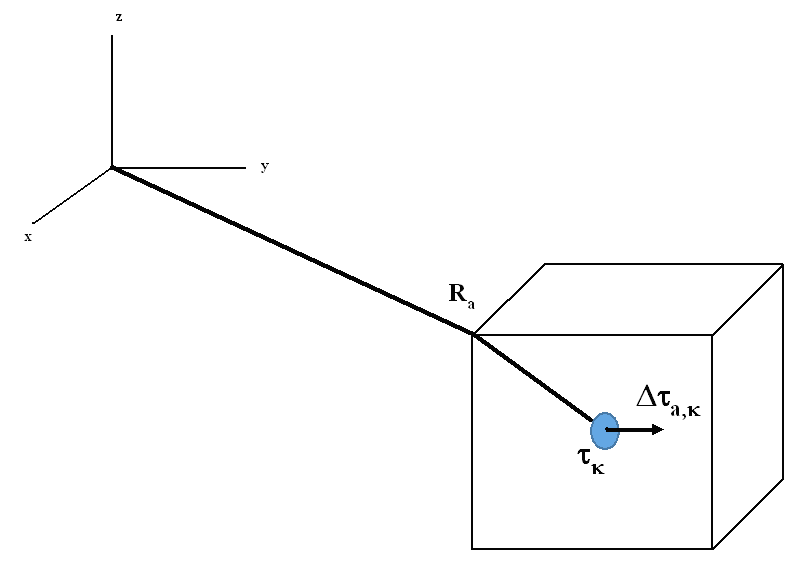
\includegraphics[scale=0.7]{figsolid}
	\caption[Reperer des atomes de la maille par rapport l'axe de coordonnées]{Chaque maille unitaire est repérée par un vecteur $R_{a}$, où a=1, 2, $\dotsc$, N. Les atomes de la maille sont repérés par $\tau_{\kappa}$ et leur déplacement par $\Delta\tau_{\kappa}$ ($\kappa$ variant de 1 à r)}
\end{figure}

Intéressons- nous maintenant au cas particulier d'un cristal, c'est-à-dire d'un solide périodique composé de N mailles élémentaires contenant r atomes par cellule unité. Alors, l'indice $\kappa$ utilisé jusqu'à présent est remplacé par le couple (a,$\kappa$). Ainsi, la position d'équilibre de l'atome $\kappa$ dans la maille a est donnée par :

\begin{equation}
R_{a\kappa}^{0}= R_{a} + \tau_{\kappa}
\end{equation}
où $R_{a}=a_{1}x_{1} + a_{2}x_{2} + a_{3}x_{3}$ est un vecteur de translation du réseau cristallin (les vecteurs $x_{i}$ étant les vecteurs primitifs du réseau direct) et $\kappa = 1, 2,\ldots,r$ désignant les atomes de la maille unitaire. Chaque atome peut se déplacer de sa position d'équilibre d'une quantité $\Delta\tau_{a,\kappa}$ (dépendant à la fois de $\kappa$ et de a) de sorte que sa position instantanée est donnée par :

\begin{equation}
R_{a,\kappa} = R_{a}+ \tau_{\kappa} + \Delta\tau_{a,\kappa}\\
= R^{0}_{a,\kappa} + \Delta\tau_{a,\kappa}
\end{equation}

Pour calculer les phonos, c'est-à-dire les fréquences propres de vibration, nous ferons l'hypothèse d'un cristal périodique infini. En d'autres termes, nous négligerons les effets de surface. Un problème survient cependant : une infinité de valeurs seront nécessaires à la description des propriétés du cristal. Nous serons ainsi amené à imposer des conditions limites périodiques, nous permettant de traiter un cristal de volume fini répété de manière périodique. 

Le problème n'est plus alors de résoudre une infinité d'équations du mouvement mais un ensemble de 3r équations homogènes dont les inconnues sont les vecteurs propres de polarisation $\eta_{\kappa,\alpha}$ (définis plus loin) et ce, pour un ensemble infini de vecteurs q de la première zone de Brillouin. En pratique, on doit se restreindre à un ensemble fini de vecteurs q. Cela correspond à imposer des conditions limites périodiques de Born von Karman, non plus sur un cristal infini mais sur un cristal fini:

\begin{equation}
\tau_{\kappa}(R_{a} + N_{i}x_{i}) = \tau_{\kappa}(R_{a})
\end{equation}

pour chacun des trois vecteurs primitifs $x_{i}$ et où les $N_{i}$ sont des nombres entiers satisfaisant la relation $N=N_{1}N_{2}N_{3}$, limitant de ce fait le nombre de vecteurs q permis dans la zone de Brillouin :

\begin{equation}
q= \frac{n_{1}}{N_{1}}b_{1}+ \frac{n_{2}}{N_{2}}b_{2}+ \frac{n_{3}}{N_{3}}b_{3}, \; \; \; \;     n_{i}  entiers
\end{equation}

En pratique on se limite  à $N_{i} =2$ ou 3. Nous avons vu que la dynamique du réseau était déterminée par l'energie de Born- Oppenheimer $E_{BO}(\{R_{a,\kappa}\})$. Dorénavant, nous désignerons cette energie par $E_{BO}(\{\Delta\tau_{a,\kappa}\})$ étant donné que les positions d'équilibre des atomes donnent une contribution constante  à l'energie et que nous ne nous intéressons qu'aux propriétés dynamiques qui ne font intervenir que les déplacements. Nous supposerons les déplacements atomiques suffisamment faibles de manière à pouvoir utiliser l'approximation harmonique\cite{}. En absence de champ électrique macroscopique, l'énergie de BO s'écrit:

\begin{equation}
E_{BO}^{harm}(\Delta\tau) = \sum_{\alpha\kappa} \left(\frac{\partial E_{BO}}{\partial\tau_{\kappa\alpha}}\right)_{0} \Delta\tau_{\kappa\alpha} + \frac{1}{2} \sum_{a,\kappa,\alpha b} \sum_{,\kappa',\beta} \left(\frac{\partial^{2}E_{BO}}{\partial\tau_{a,\kappa,\alpha}\partial\tau_{b,\kappa',\beta}}\right)_{0} \Delta\tau_{a,\kappa,\alpha}\Delta\tau_{b,\kappa',\beta}
\end{equation}

où $\alpha$ et $\beta$ sont des indices se rapportant aux trois directions de l'espace. Le terme du premier ordre est nul car nous nous sommes placés aux positions d'équilibre. La dérivée seconde est évaluée aux positions d'équilibre (indice 0). En reprenant les notations introduites précédemment, on définit alors: 

\begin{equation}
C_{\kappa,\alpha\kappa'\beta}(a,a') = \frac{\partial^{2}E_{BO}}{\partial\tau_{a,\kappa,\alpha}\partial\tau_{b,\kappa',\beta}}
\end{equation}

Ces coefficients sont appelés les constantes de force interatomiques. 

\subsection{Calcul du spectre de phonons au point $\Gamma$}

Dans tout ce qui va suivre, et quelque soit le système considéré, dans le cadre de cette thèse, nous avons calculé le spectre de phonons uniquement au centre de la zone de Brillouin (point $\Gamma$). Il est par conséquent utile de préciser les propriétés de ce point. 


Les caractéristiques du problème au point $\Gamma$ $(\overrightarrow{q}= 0)$ sont intéressantes et spécifiques par certains aspects :

\begin{itemize}
	\item[\textbullet] La matrice W$(\overrightarrow{q})$ qui est la matrice regroupant l'ensemble des valeurs propres $\omega_{m}(\overrightarrow{q})$ est plus simple à calculer au point $\Gamma$ qu'aux autres points du réseau réciproque, toutes les opérations de symétrie étant présentes en ce point. Ce qui permet:
	\begin{itemize}
	\item de réduire le nombre de calculs explicites de dérivées à un minimum;
	\item de factoriser la matrice W$(\Gamma) = W(0)$ avant la diagonalisation;
	\item d'éliminer les trois modes acoustiques.	
	\end{itemize}
	
	\bigskip
	
\item[\textbullet] En effet, une propriété unique au point $(\Gamma)$, qui n'as pas d'équivalence  dans la théorie des bandes, est que trois des modes ont une fréquences nulle, car ils correspondent aux translations pures du cristal entier. En fait, il est possible de les négliger (il est à noter que le fait d'imposer des conditions aux limites périodiques exclu la possibilité de décrire les modes rotationnels de l'ensemble du cristal).
\bigskip

\item[\textbullet] W(0) possédant toute la symétrie ponctuelle du cristal, elle peut alors être factorisée selon les représentations irréductibles du groupe ponctuel correspondant.
\bigskip

\item[\textbullet] Les modes du point $(\Gamma)$ sont les seuls qui peuvent interagir avec les ondes électromagnétiques, permettant d'atteindre les spectres IR ou Raman. 
\bigskip

\item[\textbullet] Un traitement spécifiques est requit pour le calcul des fréquences en ce point pour les semi-conducteurs polaires et les isolants. 
\bigskip

\item[\textbullet] A l'aide de l'approche en super maille, la résolution du problème au point $\Gamma$ permet l'étude des vibrations aux autres points $\overrightarrow{q}$. Cependant, cet aspect n'ayant pas été abordé lors de ma thèse, il ne sera pas traité ici. 
\end{itemize}

\end{document}

